% vim: set wrap

Below is a size 8 board with a size 5 board embedded in it. Size 5 is great for learning to play, while size 8 is played by more experienced players. It can be printed and played with small Go stones, or by marking the squares with different colour pens or pencils. Have fun playing!


\newpage

\thispagestyle{empty}

%\begin{center}
\vspace*{-17mm}
\hspace{-31mm}
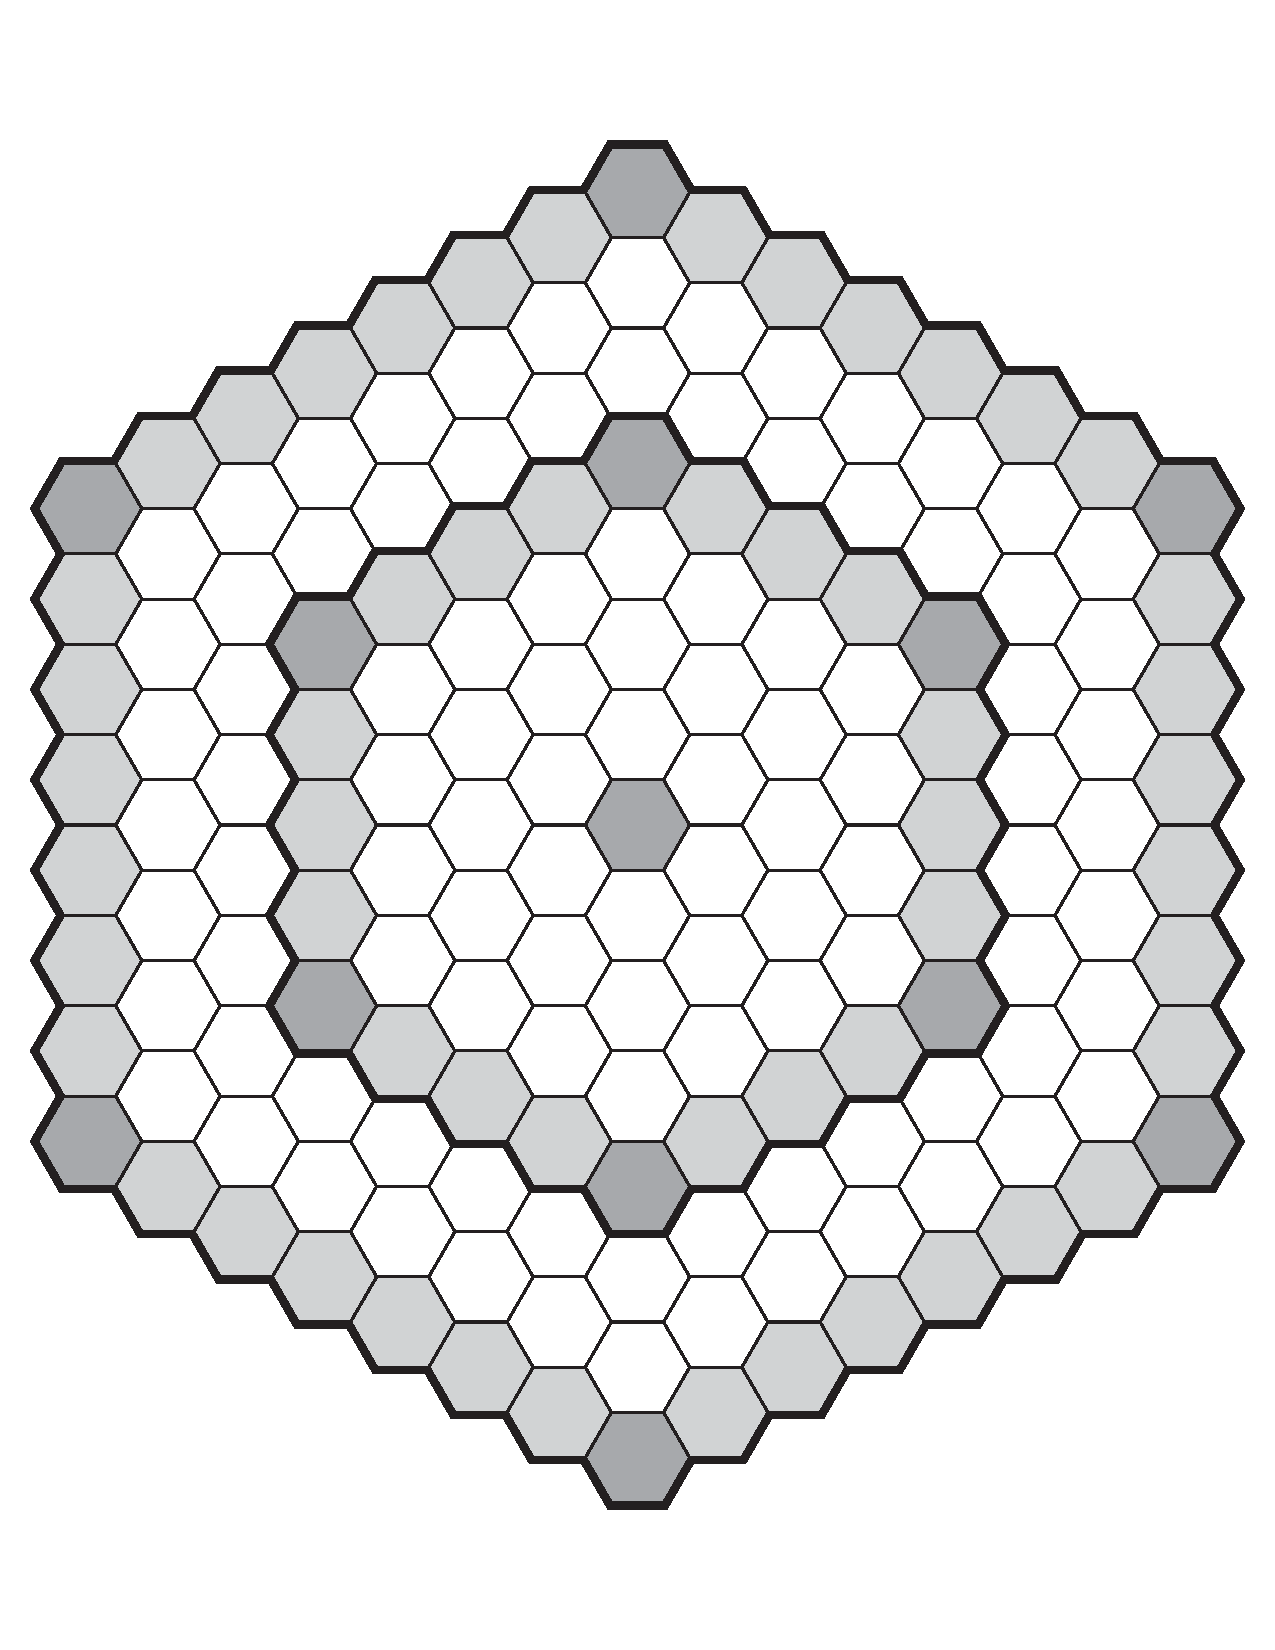
\includegraphics[width=200mm,clip=true,trim= 15pt 68pt 15pt 68pt]{boardsize8}
%width=\linewidth,
%\end{center}

%\centering
%\begin{HavannahBoard}[board size=4,coordinate style=classical,hex height=2.4cm]
%\end{HavannahBoard}

%\begin{HavannahBoard}[board size=5,coordinate style=classical,hex height=2cm]
%\end{HavannahBoard}

%\begin{HavannahBoard}[board size=6,coordinate style=classical,hex height=1.5cm]
%\end{HavannahBoard}

%\begin{HavannahBoard}[board size=7,coordinate style=classical,hex height=1.2cm]
%\end{HavannahBoard}

%\begin{HavannahBoard}[board size=8,coordinate style=classical,hex height=1cm]
%\end{HavannahBoard}

